\chapter{Introduzione}

\label{Chapter1}

La sicurezza informatica è una tra le varie tematiche più discusse oggigiorno, non solo perchè ha acquisito maggiore importanza l'informazione, ma anche per l'aumento dell'interconnessione dei vari dispositivi. È infatti possibile ottenere o inviare una risorsa da/ad una persona situato dall'altra parte del mondo, condividere in tempo reale i nostri pensieri, esperienze e tant'altro. La cosa più interessante da osservare però è come i \emph{device} o i servizi che utilizziamo quotidianamente proteggano le nostre informazioni, impedendo o meno ad altre persone esterne di accedervi. Nessuno sarebbe contento di sapere che un'altra persona, tramite vari attacchi possibili in rete, è entrata in possesso di dati privati che concernono la propria vita, come la password del proprio conto in banca o la lista dei nostri impegni.
Fortunatamente, per la maggior parte degli sviluppatori è diventato di vitale importanza valorizzare tutto il lato di sicurezza di un sistema prima di fornire un servizio, al fine di garantire all'utente riservatezza ed integrità dei propri dati.

È in questo scenario che nasce \emph{Linux Kernel Runtime Guardian}, un software innovativo con l'obiettivo di mantenere integre e sicure determinate aree del proprio sistema. Prima di parlare della sua struttura e funzionamento, è necessario introdurre gli argomenti teorici inerenti, ovvero le principali componenti di un sistema operativo (nel nostro caso Linux) e le funzionalità che un utente può utilizzare per l'interazione con esso.

%----------------------------------------------------------------------------------------
%	KERNEL
%----------------------------------------------------------------------------------------
\section{Introduzione al kernel}

Molto spesso in informatica i termini \emph{kernel} e \emph{sistema operativo} vengono utilizzati come sinonimi, perchè effettivamente il kernel è il cuore di un sistema operativo, ed ha come obiettivi principali l'interazione con le componenti hardware (hard disk, lettore DVD, etc.) e la fornitura di un ambiente per eseguire le applicazioni utente installate nel sistema.
È inoltre uno tra i primi programmi caricati durante la fase di accensione, senza il quale non sarebbe possibile l'utilizzo delle componenti fisiche.

Il primo kernel Linux è stato sviluppato da Linus Torvald nel 1991, pensato per un'architettura specifica. Negli anni la community di sviluppatori si è ampliata, rendendolo portabile e potente, capace di competere con i più grandi marchi del mercato (Windows, MacOs, etc.). Le sue principali caratteristiche sono:

\begin{itemize}
\item kernel monolitico: è un unico, grande e complesso programma composto da differenti componenti logiche;
\item caricamento dinamico dei moduli: nonostante sia un programma compilato e già in esecuzione nel sistema, offre l'opportunità di caricare/eliminare dinamicamente i moduli (noti come \emph{device driver}), le componenti che lo formano;
\item kernel threading: sono thread (un modo per dividere il programma in più componenti simultanee) del kernel associati ad un programma utente o a qualche funzionalità che Linux utilizza in maniera limitata ed efficiente per eseguire alcuni controlli periodici;
\item supporto per applicazioni multi-thread: supporta come la maggior parte dei sistemi operativi le applicazioni multi-thread;
\item preemptive: può arbitrariamente interrompere l'esecuzione di un task per poi riprenderla in seguito;
\item supporto per sistemi multi-processore: supporta \emph{SMP (symmetric multiprocessing)}, grazie al quale il sistema utilizza più processori, ognuno dei quali gestisce i propri task;
\item Virtual File System: implementando questa tecnologia, è più semplice rispetto agli altri sistemi operativi importare un \emph{file system} (componente logica per il controllo di come e dove le informazioni sono salvate) esterno.
\end{itemize}
L'attributo sul quale vale la pena fare una riflessione ai fini di questo elaborato è il caricamento dinamico dei moduli. Nonostante sia una caratteristica tipica dei sistemi basati su \emph{microkernel}, ovvero sistemi nei quali il kernel è suddiviso in vari servizi nello spazio utente (piuttosto che essere un unico software in esecuzione nello spazio kernel), Linux offre la possibilità di estendere o ridurre le funzionalità del kernel attraverso semplici strumenti.

È sufficiente utilizzare il comando \emph{modprobe} o \emph{insmode} con i privilegi di root (richiesti appunto per operazioni di rilevante importanza) per poter caricare un modulo compilato, al contrario \emph{rmmod} per rimuoverlo. Mentre insmode carica nel kernel il modulo d'interesse senza eseguire controlli di dipendenze tra moduli, modprobe carica anche tutti i moduli richiesti necessari per il corretto funzionamento.
Di seguito, ecco un esempio d'uso di alcuni di questi comandi:

\begin{lstlisting}[
	language=bash,
	basicstyle=\color{black}\ttfamily,
	backgroundcolor=\color{white}]
prova@prova:~$ sudo insmod testModule.ko
[sudo] password for prova:
prova@prova:~$ lsmod | grep testModule
Module
testModule	16384	0
prova@prova:~$ sudo rmmod testModule.ko
prova@prova:~$ lsmod | grep testModule
prova@prova:~$ 
\end{lstlisting}
È possibile osservare come una volta caricato con successo, il modulo appaia nella lista di quelli attualmente in esecuzione nel kernel (comando \emph{lsmod}). Nelle prossime sezioni verrà spiegato come un utente si può interfacciare con un modulo, leggendo l'output che esso produce o modificando determinati parametri.

\subsection{Architettura di un modulo}
Il linguaggio di programmazione utilizzato per creare un modulo è il C, con qualche differenza rispetto ai classici programmi che si è abituati a scrivere. Infatti, mentre tutti i programmi utente scritti in C richiedono che ci sia una funzione \emph{main}, nel sorgente del modulo bisogna specificare due funzioni: una di inizializzazione e una di uscita.
A scelta dello sviluppatore ma altamente consigliato per creare una buona documentazione, possono essere indicate informazioni quali la licenza, l'autore, la descrizione e una versione del modulo. Tali attributi possono essere consultati una volta compilato il modulo con il comando \emph{modinfo module\_name}.
Una volta compilato tramite un apposito \emph{makefile}, ovvero un file contenente una serie di direttive per la compilazione, si ottiene la versione \emph{.ko} del sorgente in formato ELF (Executable and Linkable Format), la quale può essere caricata con i metodi illustrati.

Osserviamo un esempio di un modulo per avere un'idea più precisa:

\begin{lstlisting}[
	language=C,
  	keywordstyle=\bfseries\color{green!40!black},
  	commentstyle=\itshape\color{purple!40!black},
  	identifierstyle=\color{blue},
  	stringstyle=\color{orange},
    basicstyle=\scriptsize\ttfamily,
    breaklines=true]
#include <linux/module.h>
#include <linux/kernel.h>
#include <linux/init.h>

static int __init hello_init(void)
{
	printk(KERN_INFO "Hello world!\n");
	return 0;
}

static void __exit hello_exit(void)
{
	printk(KERN_INFO "Goodbye World!\n");	
}

module_init(hello_init);
module_exit(hello_exit);

MODULE_LICENSE("GPL");
MODULE_AUTHOR("Simone Magnani");
MODULE_DESCRIPTION("Hello world module!");
MODULE_VERSION("0.1");
\end{lstlisting}

Tralasciando le informazioni autoesplicative finali, in tutti i moduli sono richiamate le macro \emph{module\_init} e \emph{module\_exit} alle quali vengono passate come parametri le corrispettive funzioni di inizializzazione e terminazione. Fino alla versione 2.4 del kernel, era sufficiente dichiarare tale funzioni con i nomi \emph{init\_module} e \emph{cleanup\_module}, ma per comodità di progettazione si è scelto di introdurre le macro. Il modulo una volta caricato produce come output "Hello World", mentre "Goodbye World" è il messaggio stampato durante la fase di rimozione.

È possibile trovarsi in una situazione in cui un modulo 'A' debba utilizzare delle funzioni che, per scelta progettuale o stilistica, sono implementate nel modulo 'B'. Tutto quello che serve fare è creare un \emph{header file} nel quale è dichiarato il prototipo della funzione, includerlo nel modulo 'A' tramite la direttiva \emph{include} e aggiungere alla fine dell'implementazione della funzione nel modulo 'B' la riga \emph{EXPORT\_SYMBOL(function\_name)}. Infine, è strettamente necessario che il modulo 'B' che è una sorta di 'fornitore' della specifica sia caricato prima di 'A', altrimenti la risoluzione dei simboli fallirebbe.
Per quello che ci concerne, queste sono le poche informazioni indispensabili che servono per comprendere come funziona il kernel, nel caso volessimo consultare il sorgente del software \emph{LKRG} o scrivere un proprio modulo di utility.

\subsection{Comunicazione utente-kernel}
In questa sezione vengono trattati i vari metodi di comunicazione tra lo spazio utente e kernel, ponendo maggiore importanza nell'utilizzo del \emph{Virtual File System (VFS)} e delle \emph{sysctl}, i due metodi più comunemente utilizzati. Quest'ultimo in particolare è il principio di base su cui si basa l'interazione tra l'utente e il modulo LKRG, con il quale è possibile modificare determinati parametri del kernel.

Vi sono in linux diversi modi per interagire con il kernel, tra cui:

\begin{enumerate}
\item Virtual File System (Procfs, Sysfs, Configfs, Debugfs, Character Devices)
\item Socket based mechanism (Udp sockets, Netlink sockets)
\item Ioctl (input-output control)
\item System call
\item Kernel signaling
\item Upcall
\item Mmap
\end{enumerate}

Linux implementa il concetto di virtual file system, grazie al quale l'utente può accedere a diversi tipi di file system in maniera uniforme; inoltre a seconda dell'utilizzo è possibile montarli (renderli accessibili) liberamente senza dover rispettare alcun vincolo.
Diversi possiedono una propria interfaccia grazie alla quale è più semplice interagire, tra cui ricordiamo:

\begin{itemize}
\item /proc
\item /sys
\item /dev
\item /sys/kernel/config (a volte anche solo /config)
\item /sys/kernel/debug
\end{itemize}

Inizialmente progettato per esportare tutte le informazioni riguardanti i processi, come lo stato corrente e i file descriptor aperti, \emph{/proc} è ampliamente utilizzato per fornire dati circa:

\begin{itemize}
\item il sistema in esecuzione (CPU, memoria, interrupt, etc.);
\item i device 'ide', 'scsi' e 'tty\'s';
\item la rete, come la tabella \emph{ARP} (Address resolution Protocol), la lista delle socket utilizzate o qualche statistica.
\end{itemize}

In aggiunta, al suo interno vi è un'importante cartella denominata \emph{/proc/sys}, la quale permette di configurare numerosi parametri del sistema, ognuno rappresentato da un singolo file. Tutte le sotto cartelle e i file interni non sono implementati secondo l'interfaccia \emph{procfs}, bensì rispondono ad un meccanismo del kernel appositamente costruito chiamato \emph{sysctl}.

A differenza della filosofia dei file system, secondo la quale il kernel può modificare un file ma l'utente rimane inconscio di questa modifica fino alla prossima apertura, tramite l'utilizzo delle \emph{socket} il kernel può inviare notifiche ad un'applicazione utente in ascolto in qualsiasi momento. Vi sono 3 diverse famiglie da poter utilizzare:

\begin{itemize}
\item AF\_INET: progettate per la comunicazione in rete, è possibile utilizzare socket \emph{UDP (User Datagram Protocol)}, nonostante vi possa essere più sovraccarico di messaggi.
\item AF\_PACKET: permette all'utente di definire gli headers dei pacchetti.
\item AF\_NETLINK: specialmente progettate per la comunicazione tra utente e kernel.
\end{itemize}

Tra le varie chiamate di sistema che analizzeremo nella prossima sezione, esiste la funzione \emph{ioctl()} grazie alla quale è possibile manipolare i parametri di determinati device. È implementata come un'unica funzione, la quale effettua la multiplazione dei comandi al fine che vengano richiesti i device opportuni. Il \emph{multiplexing} si basa sul \emph{file descriptor}, un puntatore astratto a quella specifica risorsa o canale, e il numero del comando da eseguire su quel preciso device.

L'invio di segnali da parte del kernel è un approcio leggermente diverso dai classici, dato che solo il kernel può inviare segnali allo spazio utente e non vice versa. Inoltre il quantitativo di dati trasportati dai segnali è molto limitato. Esistono due tipi diversi di API nello \emph{user space}: le 'normali', le quali non trasportano dati, e le 'realtime' che trasportano fino ad un massimo di 32 bit.
Affinchè il segnale sia ricevuto, nello spazio utente è necessario registrare un'apposita funzione con il compito di essere notificata; tale funzione sarà richiamata ogni volta che il kernel invierà un segnale di quel tipo.

Grazie all'uso delle \emph{Upcall}, un modulo del kernel può invocare l'esecuzione di un programma utente nell'apposito spazio, configurando gli appositi parametri e variabili d'ambiente. Possiamo definire tale procedimento 'ad hoc', in quanto un qualsiasi utente solitamente non programma un apposito modulo per ogni programma che vuole eseguire, ma può risultare molto utile come tecnica nel caso dovesse utilizzare un programma specifico.

Infine, l'unico modo per trasferire grandi quantitativi di dati tra l'utente e il kernel senza effettuarne una copia, è il \emph{memory mapping} ('mmap', mappatura della memoria). Sostanzialmente, si definisce un'area della memoria accessibile sia al kernel che all'utente, nella quale ogni attore può scrivere o leggere i dati contenuti. La differenza con le tecniche mostrate fino ad ora, risiede nella notificazione dei cambiamenti: con mmap, quando un attore scrive dei dati nella porzione condivisa, l'altro non è a conoscenza di tali cambiamenti fino a quando non ne effettua la lettura. Nel caso non vi fossero delle politiche di lettura/scrittura, se i due attori scrivessero nel buffer senza prima 'consumare' l'informazione comunicata dall'altro, vi è una perdita di dati.

\subsection{Esempi di comunicazione}

Vengono proposti i due esempi di comunicazione più classici ampiamente utilizzati nella programmazione del kernel.
Il primo metodo sfrutta il famigerato file system /proc, creando una entry del nostro modulo non appena esso viene caricato, assegnando le funzioni di lettura e scrittura che dichiariamo; in tale modo è possibile scrivere all'interno del file e leggerne il contenuto secondo le nostre politiche, implementate nelle apposite funzioni \emph{write\_proc()} e \emph{read\_proc()}.
Questo esempio è stato testato nella versione 4.15.0.33-generic del kernel Linux.

\begin{lstlisting}[
	language=C,
  	keywordstyle=\bfseries\color{green!40!black},
  	commentstyle=\itshape\color{purple!40!black},
  	identifierstyle=\color{blue},
  	stringstyle=\color{orange},
    basicstyle=\scriptsize\ttfamily,
    breaklines=true]
#include <linux/module.h>
#include <linux/kernel.h>
#include <linux/proc_fs.h>
#include <linux/sched.h>
#include <linux/uaccess.h>
#include <linux/slab.h>
#define MSG_SIZE (512)

static char *msg;
static int len,tmp;

ssize_t write_proc(struct file *filp, const char *buf, size_t count, loff_t *offp)
{
    unsigned long actual_len = count < MSG_SIZE - 1 ? count : MSG_SIZE - 1;
    copy_from_user(msg, buf, actual_len);
    len = count;
    tmp = len;
    return len;
}

ssize_t read_proc(struct file *filp, char *buf, size_t count, loff_t *offp)
{
    if(count > tmp) 
        count = tmp;
    tmp = tmp - count;
    copy_to_user(buf, msg, count);
    if(count == 0)
        tmp = len;
    return count;
}

struct file_operations proc_fops =
{
write:
    write_proc,
read:
    read_proc
};

static int __init proc_init(void)
{
    if ((msg = kmalloc(MSG_SIZE, GFP_KERNEL)) == NULL)
        return -ENOMEM;
    proc_create("myProc", 0, NULL, &proc_fops);
    return 0;
}

static void __exit proc_exit(void)
{
    remove_proc_entry("myProc", NULL);
    kfree(msg);
}

MODULE_LICENSE("GPL");
module_init(proc_init);
module_exit(proc_exit);
\end{lstlisting}

Si è dichiarato un buffer denominato \emph{msg} il quale ha il compito di tenere in memoria il contenuto della nostra entry \emph{myEntry}. Nella struttura \emph{file\_operations}, sono state agganciate le nostre rispettive funzioni di write e read, le quali non fanno altro che copiare il messaggio utente in msg nel primo caso,  viceversa nel secondo.
È molto importante eliminare la entry e liberare la memoria allocata per il nostro buffer quando il modulo viene rimosso, onde evitare errori o sprechi inutili di memoria.
Una volta caricato nel kernel, per interagire con il nuovo file /proc/myEntry è sufficiente utilizzare dei semplici comandi \emph{cat} e \emph{echo} come di seguito:

\begin{lstlisting}[
	language=bash,
	basicstyle=\color{black}\ttfamily,
	backgroundcolor=\color{white}]
prova@prova:~$ sudo insmod proc_entry.ko
[sudo] password for prova:
prova@prova:~$ lsmod | grep proc_entry
Module
proc_entry	16384	0
prova@prova:~$ echo "Ciao Mondo" > /proc/myEntry
prova@prova:~$ cat /proc/myEntry
Ciao Mondo
prova@prova:~$ 
\end{lstlisting}

Il secondo esempio proposto sfrutta la funzionalità \emph{sysctl} del kernel, con la quale è possibile modificare determinati parametri a runtime sfruttando la directory /sys all'interno del file system /proc. 

\begin{lstlisting}[
	language=C,
  	keywordstyle=\bfseries\color{green!40!black},
  	commentstyle=\itshape\color{purple!40!black},
  	identifierstyle=\color{blue},
  	stringstyle=\color{orange},
    basicstyle=\scriptsize\ttfamily,
    breaklines=true]
#include <linux/module.h>
#include <linux/kernel.h>
#include <linux/sysctl.h>

int my_var = 0;

static struct ctl_table_header *my_header;

static struct ctl_table my_value[] =
{
    {
        .procname       = "my_value",
        .data           = &my_var,
        .maxlen         = sizeof(int),
        .mode           = 0600,
        .proc_handler   = proc_dointvec_minmax,
    },
    {}
};

static struct ctl_table my_directory[] =
{
    {
        .procname    = "example",
        .mode        = 0600,
        .child       = my_value,
    },
    { }
};

static int __init myInit(void)
{
    /* register the above sysctl */
    my_header = register_sysctl_table(my_directory);
    if (!my_header)
        return -EFAULT;
    return 0;
}

static void __exit myExit(void)
{
    unregister_sysctl_table(my_header);
}

MODULE_LICENSE("GPL");
module_init(myInit);
module_exit(myExit);
\end{lstlisting}

Il modulo crea una propria directory (all'interno di /proc/sys/) chiamata `example` con all'interno l'attributo \emph{my\_value}, al cui cambiamento viene risettato il valore della variabile \emph{my\_var} (il nostro "parametro" del kernel). Configurata la directory, viene registrata all'interno della tabella delle sysctl, e viene ritornato l'header a questa struttura, il quale serve non solo per verificare se l'operazione è andata a buon fine, ma anche per rimuovere l'entry dalla tabella delle sysctl durante la rimozione del modulo.
Di seguito viene mostrato un'esempio d'uso del comando \emph{sysctl} con il nostro parametro registrato:

\begin{lstlisting}[
	language=bash,
	basicstyle=\color{black}\ttfamily,
	backgroundcolor=\color{white}]
prova@prova:~$ sudo insmod sysctl.ko
[sudo] password for prova:
prova@prova:~$ lsmod | grep sysctl
Module
sysctl	16384	0
prova@prova:~$ sysctl -a | grep my\_value
example.my_value = 0
prova@prova:~$ sysctl example.my\_value=100
example.my_value = 100
prova@prova:~$ sysctl -a | grep my\_value
example.my_value = 100
\end{lstlisting}

Un ultimo dettaglio su questo strumento: l'entry aggiunta al file system /proc viene rimossa al successivo riavvio della macchina, a meno che non vengano aggiunte queste preferenze al file \emph{/etc/sysctl.conf}.

%----------------------------------------------------------------------------------------
%	ARCHITECTURE
%----------------------------------------------------------------------------------------
\section{Architettura di un processore}

L'idea di porre dei livelli gerarchici di protezione processore e della memoria (cosiddetti \emph{ring}), è stata per la prima volta introdotta nel computer \emph{GE 645} nel 1965. Questa innovazione è stata molto apprezzata e rivisitata dalla maggior parte dei concorrenti nel mondo informatico, ed è persino utilizzata tutt'ora, seppure con qualche modifica.\\\\
L'idea consiste nell'inserire dei controlli riguardanti l'accesso al processore, per proteggere il sistema in base alla tipologia di operazione che deve svolgere. Tali controlli possono essere implementati in 3 modi:

\begin{itemize}
\item hardware(HW): i livelli di privilegi sono implementati in microcodice HW per il controllo degli accessi;
\item software(SW): il meccanisco di controllo è interamente a livello SW;
\item hardware + software (ibridi): componenti di entrambe le nature collaborano nella gestione dei ring.
\end{itemize}

Generalmente i sistemi con i controlli ibridi sono ottenuti combinando componenti progettate appositamente per tale funzionamento. Supponiamo di avere un computer con il processore strutturato per la cooperazione con un sistema operativo che, diversamente, implementa i controlli solamente a livello software. Cosa succede? Sicuramente potremmo affermare di non avere una gestione dei livelli sia software che hardware, in quanto nel sistema non è integrata questa funzionalità.

Il numero di ring può variare, ma generalmente quelli più interessanti da sapere che sono presenti in tutte le implementazioni sono due: livello 0 (kernel mode) e livello utente (user mode). Mentre il livello 0 è utilizzato dal sistema operativo e rappresenta la massima affidabilità, il livello utente è il livello meno privilegiato, dal quale il sistema si aspetta che le operazioni possano essere malevole.

\begin{figure}[!ht]
\centering
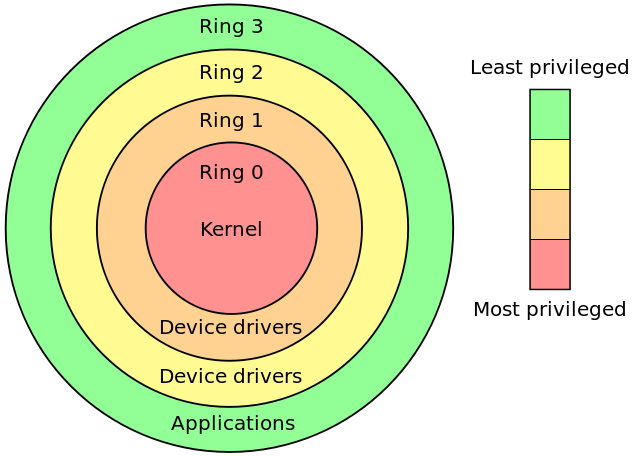
\includegraphics[scale=0.3]{Figures/RingCpu}
\caption[Ring nei processori della famiglia x86]{Ring nei processori della famiglia x86.\\Fonte: \href{https://en.wikipedia.org/wiki/Protection_ring}{https://en.wikipedia.org}}
\label{fig:RingCpu}
\end{figure}

Si può notare in \autoref{fig:RingCpu} che tra i due livelli appena discussi ve ne sono altri due utilizzati dai \emph{device drivers}, ossia da quei programmi che controllano e gestiscono determinati dispositivi fisici o virtuali collegati al calcolatore. Un esempio molto comune è l'installazione della propria stampante a casa: quando viene richiesto di scaricare/aggiornare i driver, si tratta di queste risorse che si interfacciano con il dispositivo fisico.

\subsection{User/Kernel spaces}

La memoria di un calcolatore è suddivisa in due importanti aree: \emph{user space} (spazio utente) e \emph{kernel space} (spazio kernel).

Con il termine user space si fa riferimento a tutto il codice eseguito al di fuori del kernel del sistema operativo. Ogni processo eseguito in questo spazio ha una propria memoria virtuale e non può comunicare, a meno che non venga esplicitato attraverso varie tecniche di programmazione, con gli altri processi. È importante sottolineare che un processo nello spazio utente non ha completo accesso alle risorse di sistema; l'utilizzo di tali risorse è garantito dalle varie \emph{API (Application Programming Interface)} messe a disposizione dal sistema.

Il kernel space ha la proprietà di eseguire il codice a livello 0, tipicamente definita esecuzione in kernel mode. In tale modalità, i processi godono del completo accesso all'hardware e alle risorse, in quanto sono considerati affidabili.

\begin{figure}[!ht]
\centering
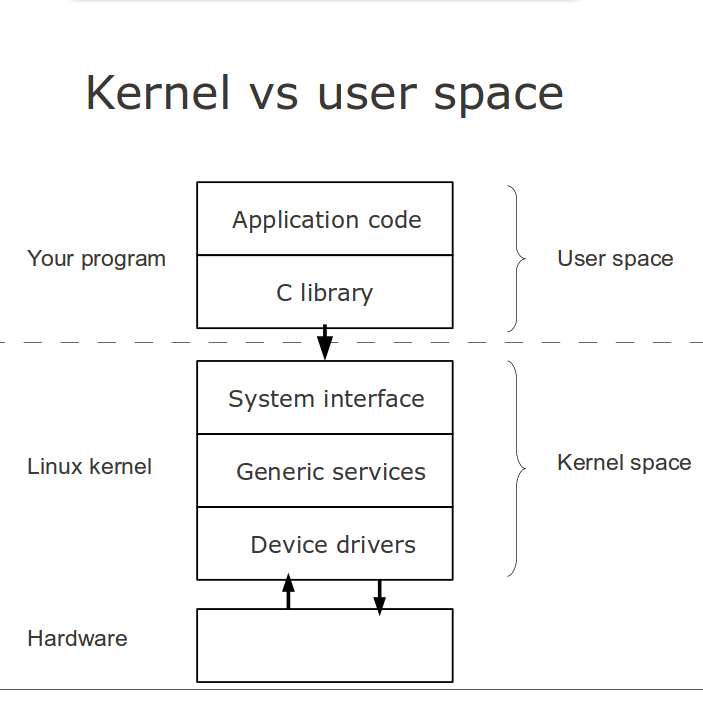
\includegraphics[scale=0.3]{Figures/Spaces}
\caption[Kernel space e User space]{Kernel space e User space.\\ Fonte: \href{https://3.bp.blogspot.com/-s-8vrCL_OPg/V33EJafdJTI/AAAAAAAAPcY/rKlsSv2ay-IYRHLoZdKS07YIgPVS9JX9QCLcB/s1600/Screenshot+from+2016-07-07_08-18-32.png}{https://3.bp.blogspot.com}}
\label{fig:KUSpace}
\end{figure}

La \autoref{fig:KUSpace} rappresenta i due diversi livelli di spazio e come si interfacciano con l'hardware.
Supponiamo di dover lanciare un programma C che esegue una semplice operazione di scrittura su disco (ad esempio salvataggio di un file) per poi terminare. Come discusso poco fa, l'esecuzione del nostro programma avviene nello user space, ovvero lo spazio dove l'accesso diretto all'hardware non è permesso onde evitare danni alle risorse. L'eseguibile dovrà pertanto effettuare una richiesta (detta anche segnalazione) al sistema grazie alla quale avviene la scrittura su disco. Come è possibile che sia avvenuta l'operazione nonostante il mio programma è eseguito nello spazio utente in modalità utente?
Quando il programma ha inviato la segnalazione al sistema, la \emph{CPU (Control Processor Unit)} ha effettuato un'operazione di scambio molto importante tra il ring 0 ed il ring utente grazie alla quale in nostro programma riesce a terminare con successo: il \emph{mode switch}.

\subsection{CPU mode switch}

Talvola il termine \emph{mode switch} viene confuso con \emph{context switch}, sebbene siano due cose concettualmente diverse. Mentre con il secondo si indica il passaggio effettuato dallo scheduler della CPU da un processo o thread ad un altro, il mode switch è il cambio di modalità di esecuzione delle istruzioni all'interno dello stesso processo. Quando il programma utente effettua una segnalazione di sistema per richiedere l'utilizzo di determinato hardware, all'interno della CPU avviene un cambio di modalità, passando dall'esecuzione in modalità utente alla modalità kernel. Avendo ora i privilegi necessari, è possibile soddisfare la richiesta e, una volta terminata, verrà effettuato un ulteriore passaggio per ritornare alla modalità utente.

Il mode switch e il context switch a seconda di come sono implementati possono avere un costo di esecuzione in termine di tempo molto variabile. Per questo si cerca di progettare il sistema operativo in maniera da effettuare il minor numero di passaggi che, nonostante avvengano in tempi pari all'ordine del nanometro, sono impercettibili all'essere umano ma non trascurabili per il processore.
Uno dei vantaggi da sempre riconosciuto a Linux è proprio quello di aver un costo estremamente basso per effettuare tali operazioni.

\section{Le system call}

Fino ad ora si è parlato di interfacce per segnalare al sistema la richiesta di un'istruzione privilegiata senza spiegare altro. Queste funzioni sono conosciute con il nome di \emph{system call (chiamate di sistema)} e sono presenti in ogni sistema operativo, sebbene in maniera differente. Infatti tali funzioni non sono universali per problemi di incompatibilità sia hardware che software; ogni sistema operativo ne possiede delle proprie, le quali hanno comunque come unico obiettivo l'interazione del programma con il sistema e i device che ne fanno parte.

\begin{figure}[!ht]
\centering
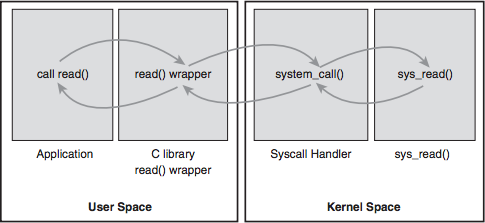
\includegraphics[scale=0.7]{Figures/Syscall}
\caption[Esempio di system call read()]{Esempio di system call read().\\ Fonte: \href{https://www.quora.com/How-does-System-Call-return-data-back-to-user-space-in-Linux-Kernel}{https://www.quora.com}}
\label{fig:Syscall}
\end{figure}

La \autoref{fig:Syscall} mostra un esempio di chiamata della system call \emph{read()}: tra la chiamata a funzione nella nostra applicazione e la vera chiamata di sistema, si noti come è presente un \emph{call wrapper}. Un wrapper consiste in un \emph{layer} di codice con il compito di tradurre in un'interfaccia compatibile il codice di libreria; è sostanzialmente un API grazie alla quale non vi è bisogno di reimplementare del codice, ma si utilizza l'interfaccia che tale prodotto mette a disposizione.
La chiamata \emph{read()} è in realtà un'invocazione del wrapper presente nella libreria standard del linguaggio C (\emph{glibc}), il quale ha il compito a sua volta di richiamare la vera e propria system call.
Una volta invocata ed avvenuto il \emph{mode switch} in quanto deve essere eseguito del codice kernel, un \emph{handler} (intercettatore) inoltra la chiamata ad un livello inferiore, oltre al quale avviene l'operazione vera e propria sul device (fisico o virtuale) d'interesse. Alla fine dell'operazione, la CPU ritorna in modalità utente ed il controllo viene restituito al programma.

Una lista completa di tutte le system call con documentazione può essere trovata nel sito \url{http://man7.org/linux/man-pages/man2/}.

\subsection{Esempi di strumenti utili}
In questa sezione vengono mostrati brevemente degli strumenti da riga di comando molto utili per la fase di debugging del nostro programma, nel caso fossimo interessati a comprenderne il funzionamento a più basso livello.
Supponiamo di avere il nostro programma C come segue:

\begin{lstlisting}[
  	language=C,
  	keywordstyle=\bfseries\color{green!40!black},
  	commentstyle=\itshape\color{purple!40!black},
  	identifierstyle=\color{blue},
  	stringstyle=\color{orange},
    basicstyle=\scriptsize\ttfamily,
    breaklines=true,
    escapechar=\!]
#include <fcntl.h>

int main(void)
{
	int fd = open("foo.txt", O\_RDONLY);
	if(fd > 0) close(fd);
	return 0;
}
\end{lstlisting}

Nella funzione main viene dichiarato un intero all'interno del quale verrà salvato il file descriptor di \emph{foo.txt} nel caso il file esista, altrimenti -1. Se l'apertura del file è avvenuta con successo, si prosegue con la semplice chiusura.
Le funzioni \emph{open()} e \emph{close()} sono delle chiamate di sistema, le quali comunicano al kernel di eseguire tali operazioni privilegiate nell'hardware.
Grazie al comando \emph{strace} è possibile visualizzare tutte le system call effettuate dal nosto programma. Lanciando il comando \emph{strace ./myprogram} dove \emph{myprogram} è l'eseguibile ottenuto in seguito alla compilazione, si ottiene un output simile:

\begin{lstlisting}[
  	language=C,
  	basicstyle=\scriptsize\ttfamily\color{black},
    backgroundcolor=\color{white},
    breaklines=true,
  	escapeinside={(*@}{@*)}]
prova@prova:~$ strace ./myprogram

execve("./myprogram", ["./myprogram"], [/* 70 vars */]) = 0
brk(0)                                  = 0x22c3000
access("/etc/ld.so.nohwcap", F_OK)      = -1 ENOENT (No such file or directory)
mmap(NULL, 8192, PROT_READ|PROT_WRITE, MAP_PRIVATE|MAP_ANONYMOUS, -1, 0) = 0x7f8feb036000
access("/etc/ld.so.preload", R_OK)      = -1 ENOENT (No such file or directory)
open("/etc/ld.so.cache", O_RDONLY|O_CLOEXEC) = 3
fstat(3, {st_mode=S_IFREG|0644, st_size=79132, ...}) = 0
mmap(NULL, 79132, PROT_READ, MAP_PRIVATE, 3, 0) = 0x7f8feb022000
close(3)                                = 0
access("/etc/ld.so.nohwcap", F_OK)      = -1 ENOENT (No such file or directory)
open("/lib/x86_64-linux-gnu/libc.so.6", O_RDONLY|O_CLOEXEC) = 3
read(3, "\177ELF\2\1\1\0\0\0\0\0\0\0\0\0\3\0>\0\1\0\0\0P \2\0\0\0\0\0"..., 832) = 832
fstat(3, {st_mode=S_IFREG|0755, st_size=1840928, ...}) = 0
mmap(NULL, 3949248, PROT_READ|PROT_EXEC, MAP_PRIVATE|MAP_DENYWRITE, 3, 0) = 0x7f8feaa51000
mprotect(0x7f8feac0b000, 2097152, PROT_NONE) = 0
mmap(0x7f8feae0b000, 24576, PROT_READ|PROT_WRITE, MAP_PRIVATE|MAP_FIXED|MAP_DENYWRITE, 3, 0x1ba000) = 0x7f8feae0b000
mmap(0x7f8feae11000, 17088, PROT_READ|PROT_WRITE, MAP_PRIVATE|MAP_FIXED|MAP_ANONYMOUS, -1, 0) = 0x7f8feae11000
close(3)                                = 0
mmap(NULL, 4096, PROT_READ|PROT_WRITE, MAP_PRIVATE|MAP_ANONYMOUS, -1, 0) = 0x7f8feb021000
mmap(NULL, 8192, PROT_READ|PROT_WRITE, MAP_PRIVATE|MAP_ANONYMOUS, -1, 0) = 0x7f8feb01f000
arch_prctl(ARCH_SET_FS, 0x7f8feb01f740) = 0
mprotect(0x7f8feae0b000, 16384, PROT_READ) = 0
mprotect(0x600000, 4096, PROT_READ)     = 0
mprotect(0x7f8feb038000, 4096, PROT_READ) = 0
munmap(0x7f8feb022000, 79132)           = 0
(*@\hl{open("foo.txt", O\_RDONLY)               = 3}@*)
(*@\hl{close(3)                                = 0}@*)
exit_group(0)                           = ?
+++ exited with 0 +++
\end{lstlisting}

Le due righe evidenziate corrispondono esattamente alle due system call richiamate nel programma C, quindi possiamo affermare che quando viene effettuata l'apertura di un file, una scrittura, una lettura o operazioni simili avviene effettivamente la chiamata di una system call con tutto il procedimento di mode switch presentato nella precedente sezione. L'esempio proposto è piuttosto banale e l'uso del comando strace in una situazione del genere è pressochè inutile, ma si immagini in un software molto più complesso quanto possa essere utile analizzare il numero di system call effettuate, al fine di stimare e/o ridurre il tempo di esecuzione in kernel mode.

Un altro comando proposto è \emph{objdump} (esistono comandi molto più potenti e interattivi, come \emph{radare} o \emph{gdb}, ma meno semplici da utilizzare), il quale permette di disassemblare l'eseguibile ed ottenere il codice in linguaggio Assembly corrispondente.
Scrivendo in un terminale \emph{objdump -d myprogram}, si comunica al tool di effettuare il disassemblaggio dell'eseguibile \emph{myprogram}. Eliminando un po' di output non interessante e concentrandoci sulla funzione \emph{main} si ottiene:

\begin{lstlisting}[
	language={[x86masm]Assembler},
	basicstyle=\scriptsize\ttfamily\color{black},
  backgroundcolor=\color{white},
	escapechar=\!]
prova@prova:~$ objdump -d myprogram
...
000000000040057d <main>:
  40057d:	55                   	push   %rbp
  40057e:	48 89 e5             	mov    %rsp,%rbp
  400581:	48 83 ec 10          	sub    $0x10,%rsp
  400585:	be 00 00 00 00       	mov    $0x0,%esi
  40058a:	bf 44 06 40 00       	mov    $0x400644,%edi
  40058f:	b8 00 00 00 00       	mov    $0x0,%eax
  400594:	e8 e7 fe ff ff       	   !\hl{callq  400480 <open@plt>}!
  400599:	89 45 fc             	mov    %eax,-0x4(%rbp)
  40059c:	83 7d fc 00          	cmpl   $0x0,-0x4(%rbp)
  4005a0:	7e 0f                	jle    4005b1 <main+0x34>
  4005a2:	8b 45 fc             	mov    -0x4(%rbp),%eax
  4005a5:	89 c7                	mov    %eax,%edi
  4005a7:	b8 00 00 00 00       	mov    $0x0,%eax
  4005ac:	e8 9f fe ff ff       	   !\hl{callq  400450 <close@plt>}!
  4005b1:	b8 00 00 00 00       	mov    $0x0,%eax
  4005b6:	c9                   	leaveq 
  4005b7:	c3                   	retq   
  4005b8:	0f 1f 84 00 00 00 00 	nopl   0x0(%rax,%rax,1)
  4005bf:	00 
\end{lstlisting}

Come nell'output precedente, sono riportate in evidenza le due chiamate di sistema \emph{open()} e \emph{close()} con le relative operazione intermedie di caricamento parametri nei registri della CPU e pulizia di registri dove salvare l'output. Per chi volesse comprendere il significato di \emph{@plt}, è possibile trovato una soddisfacente spiegazione nel seguente sito \url{https://www.technovelty.org/linux/plt-and-got-the-key-to-code-sharing-and-dynamic-libraries.html}.
Le system call e il codice assembly variano a seconda dell'architettura e del sistema operativo, quindi è molto probabile che lanciando i comandi proposti non si ottengano gli stessi risultati.
